% !TEX root = Projektdokumentation.tex


\section{Anhang}
    \subsection{Detaillierte Zeitplanung}
    \label{app:Zeitplanung}
    \begin{table}[ht]
        \tabelleAnhang{ZeitplanungKomplett}
        \caption{Detaillierte Zeitplanung}
    \end{table}
    
    \subsection{Beispielauflistung}
    \label{app:Beispielauflistung}
    Hardware
    \begin{itemize}
        \item Mobiler Arbeitsplatz (HP EliteBook 840 G5)
        \item 	Zwei Monitore
    \end{itemize}
    
    %/pagebreak
    
    \subsection{Beispielbild}
    \label{app:Excel}

    \begin{figure}[H]
        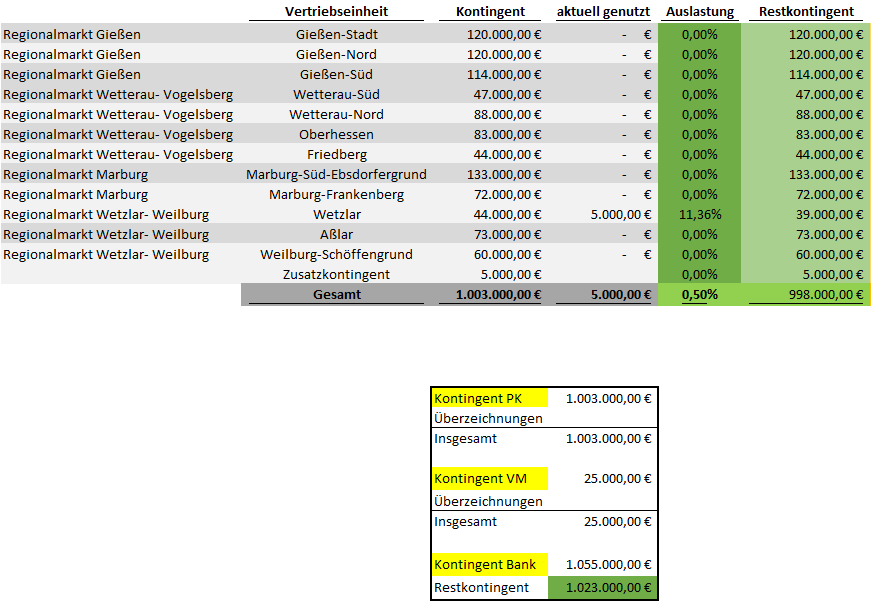
\includegraphics[width=\textwidth,height=\textheight,keepaspectratio]{images/img_exceltable.png}
        \caption{Ausschnitt Excel-Dokument}
    \end{figure}

    \subsection{Beispieltabelle}
    \label{app:Beispieltabelle}
    \begin{table}[ht]
        \tabelleAnhang{Kostenplanung}
        \caption{Kostenplanung}
    \end{table}
    
    \subsection{Berechnung}
    \label{app:Berechnung}
    
    \begin{equation}
    \label{app:BerechnungX}
        \begin{array}{1}
            Jährliche\;Zeitersparnis = 555\;Minuten/Monat\;*\; 6.660\;Minuten/Jahr = 111\;Stunden/Jahr\\
            Jährlicher\:Rückfluss = 111\:Stunden/Jahr * 60\:Euro/Stunde = 6.660 Euro\\
            Amortisationsdauer = 7.040\;Euro Kosten/6.660\;Euro Rückfluss = 1,057\;Jahre
        \end{array}
    \end{equation}

     \subsection{Code-Beispiele}
     \label{app:Codebeispiele}
         

    \subsubsection{Codebeispiel}
    \label{app:Codebeispiel}
    \definecolor{lightgrey}{rgb}{0.9,9, 0.9} % 0.8, 0.8, 1 --> lightpurple
    
        \lstset{
    	numbers=left,
    	stepnumber=1,
    	numbersep=5pt,
    	numberstyle=\small\color{black},
    	basicstyle=\ttfamily,
    	keywordstyle=\color{black},
    	commentstyle=\color{black},
    	stringstyle=\color{black},
    	frame=single,
    	tabsize=3,
    	backgroundcolor=\color{lightgrey}}
    
    \begin{lstlisting}
        var x = 12345
    \end{lstlisting}
